\documentclass{article}

\usepackage{tikz}
\usepackage[inner=0.5cm,outer=0.5cm]{geometry}

\begin{document}

\subsection*{mmm}

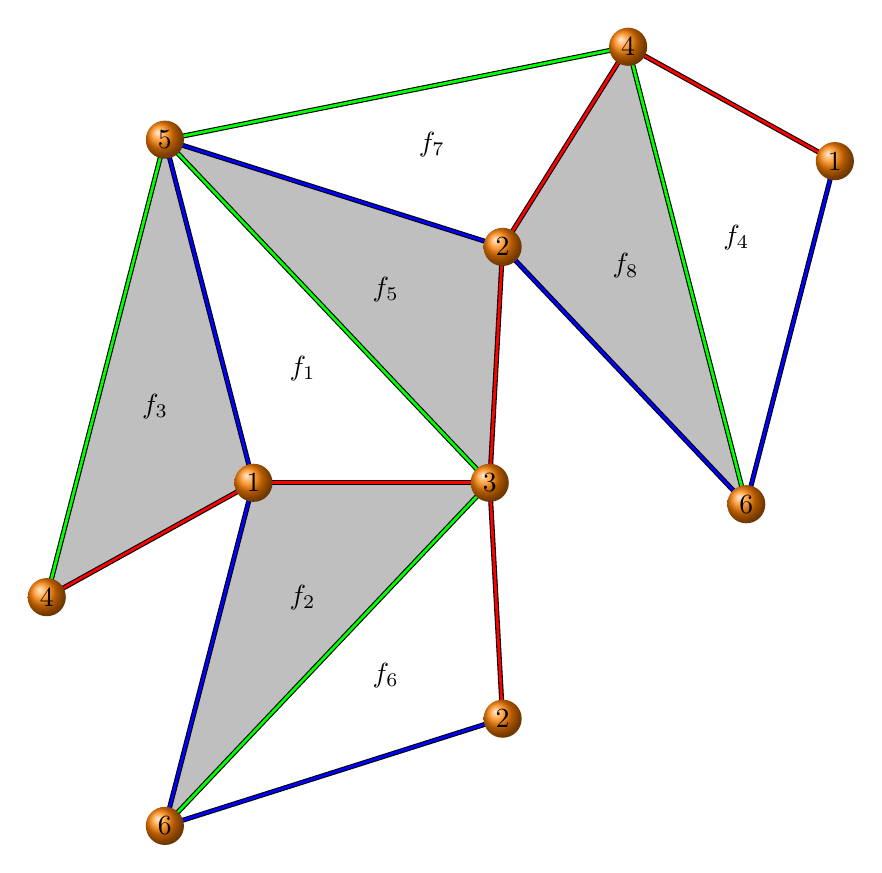
\begin{tikzpicture}[scale=3/2]
\coordinate (V1_1) at (0, 0);
\coordinate (V1_2) at (4.921875, 2.72319141530209);
\coordinate (V2_1) at (2.109375, 1.997007037888199);
\coordinate (V2_2) at (2.109375, -1.997007037888199);
\coordinate (V3_1) at (2, 0);
\coordinate (V4_1) at (-1.75, -0.9682458365518543);
\coordinate (V4_2) at (3.171875, 3.691437251853944);
\coordinate (V5_1) at (-0.75, 2.904737509655563);
\coordinate (V6_1) at (-0.75, -2.904737509655563);
\coordinate (V6_2) at (4.171875, -0.181546094353473);


\fill[white] (V1_1) -- (V3_1) -- (V5_1) -- cycle;
\node (F1) at (0.4166666666666666, 0.9682458365518543) {$f_{1}$};
\fill[lightgray] (V1_1) -- (V3_1) -- (V6_1) -- cycle;
\node (F2) at (0.4166666666666666, -0.9682458365518541) {$f_{2}$};
\fill[lightgray] (V1_1) -- (V4_1) -- (V5_1) -- cycle;
\node (F3) at (-0.8333333333333333, 0.6454972243679029) {$f_{3}$};
\fill[white] (V1_2) -- (V4_2) -- (V6_2) -- cycle;
\node (F4) at (4.088541666666666, 2.077694190934187) {$f_{4}$};
\fill[lightgray] (V2_1) -- (V3_1) -- (V5_1) -- cycle;
\node (F5) at (1.119791666666667, 1.633914849181254) {$f_{5}$};
\fill[white] (V2_2) -- (V3_1) -- (V6_1) -- cycle;
\node (F6) at (1.119791666666667, -1.633914849181254) {$f_{6}$};
\fill[white] (V2_1) -- (V4_2) -- (V5_1) -- cycle;
\node (F7) at (1.510416666666667, 2.864393933132569) {$f_{7}$};
\fill[lightgray] (V2_1) -- (V4_2) -- (V6_2) -- cycle;
\node (F8) at (3.151041666666667, 1.835632731796223) {$f_{8}$};


\tikzset{EdgeStyle/.style = {thin, double distance=1pt} }

\draw[ EdgeStyle, double=red] (V3_1) -- (V1_1);
\draw[ EdgeStyle, double=red] (V1_1) -- (V4_1);
\draw[ EdgeStyle, double=red] (V4_2) -- (V1_2);
\draw[ EdgeStyle, double=blue] (V1_1) -- (V5_1);
\draw[ EdgeStyle, double=blue] (V6_1) -- (V1_1);
\draw[ EdgeStyle, double=blue] (V1_2) -- (V6_2);
\draw[ EdgeStyle, double=red] (V2_1) -- (V3_1);
\draw[ EdgeStyle, double=red] (V3_1) -- (V2_2);
\draw[ EdgeStyle, double=red] (V4_2) -- (V2_1);
\draw[ EdgeStyle, double=blue] (V5_1) -- (V2_1);
\draw[ EdgeStyle, double=blue] (V6_2) -- (V2_1);
\draw[ EdgeStyle, double=blue] (V2_2) -- (V6_1);
\draw[ EdgeStyle, double=green] (V5_1) -- (V3_1);
\draw[ EdgeStyle, double=green] (V3_1) -- (V6_1);
\draw[ EdgeStyle, double=green] (V4_1) -- (V5_1);
\draw[ EdgeStyle, double=green] (V5_1) -- (V4_2);
\draw[ EdgeStyle, double=green] (V4_2) -- (V6_2);


\tikzset{VertexStyle/.style = {
 shape = circle,
 ball color = orange,
 text = black,
 inner sep = 2pt,
 outer sep = 0pt,
 minimum size = 10pt} }

\node[VertexStyle] at (V1_1) {1};
\node[VertexStyle] at (V1_2) {1};
\node[VertexStyle] at (V2_1) {2};
\node[VertexStyle] at (V2_2) {2};
\node[VertexStyle] at (V3_1) {3};
\node[VertexStyle] at (V4_1) {4};
\node[VertexStyle] at (V4_2) {4};
\node[VertexStyle] at (V5_1) {5};
\node[VertexStyle] at (V6_1) {6};
\node[VertexStyle] at (V6_2) {6};

\end{tikzpicture}

\end{document} 
